\documentclass[11pt,a4paper]{report}
\usepackage[utf8x]{inputenc}
\usepackage{ucs}
\usepackage{amsmath}
\usepackage{amsfonts}
\usepackage{amssymb}
\usepackage{graphicx}
\usepackage[usenames,dvipsnames]{color}
\usepackage{listings}
\usepackage{verbatim}
\usepackage[margin=2cm]{geometry}
\usepackage{asymptote}
\usepackage{tikz}
\usepackage{hyperref}
\usepackage{caption}
\usepackage{subcaption}

\definecolor{light-gray}{gray}{0.925}
\definecolor{light-gray}{rgb}{0.8,0.9,0.8}
\definecolor{no_modify}{gray}{0.925}
\definecolor{no_modify}{rgb}{0.9,0.85,0.85}

\definecolor{bordercolor}{cmyk}{1,.60,0,.40}
%\definecolor{bordercolor}{gray}{0.5}

\lstset{language=C++, 
basicstyle=\ttfamily,
keywordstyle=\color{blue}\ttfamily,
stringstyle=\color{red}\ttfamily,
commentstyle=\color{OliveGreen}\ttfamily,
morecomment=[l][\color{magenta}]{\#},
backgroundcolor=\color{light-gray}
}

\begin{asydef}
import three;
usepackage("bm");
texpreamble("\def\V#1{\bm{#1}}");
\end{asydef}


\begin{document}
\chapter{Introduction}
\emph{piccante}, the code described in this document, is a massively parallel fully-relativistic 3D particle-in-cell code. The user is able to define an arbitrary number of particle species with arbitrary density functions and an arbitrary number of Gaussian laser pulses.\\
The code is proved to run on up to 16384 MPI processes. Some preliminary scaling tests verified a very good scalability on up to 4096 MPI tasks.\\
In its present state, the code could be considered in ``beta testing''.\\
This document should provide all the information needed to compile the code, run simulations and analyse the results.
\begin{figure}[h!]
\centering
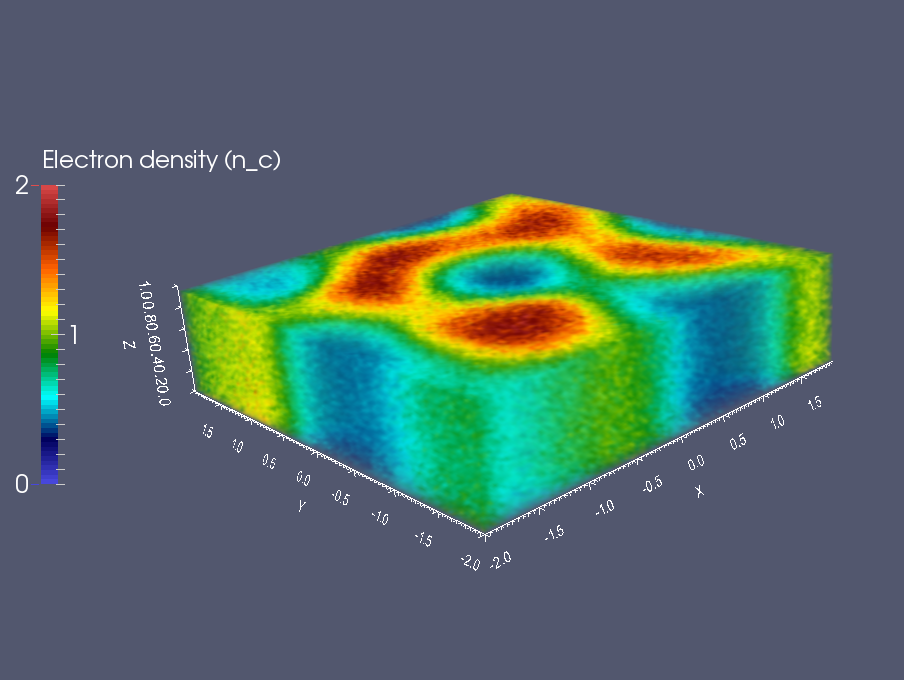
\includegraphics[width=0.9\textwidth]{3d_marta.png}
\end{figure}



\chapter{How to get and compile the code}
The following instructions describe the procedure to compile the code in a Linux system. However the code can be compiled also on a Windows system and should be compilable also on an Apple system.
\section{How to get the code} \label{section_getcode}
\subsection{Github}  
The code is distributed via an open-source repository hosted on \url{https://github.com/}.\\
Make sure that \emph{git} (a distributed version control system) is installed on your machine (\url{http://git-scm.com/}).
On a Debian-based system, just type:
\begin{verbatim}
$ sudo apt-get install git
\end{verbatim}
Once \emph{git} is installed on your system, it is possible to easily install and keep updated the code.\\
To install the code:
\begin{verbatim}
# git clone https://github.com/ALaDyn/piccante.git
\end{verbatim}
A folder named \verb+piccante+ will be created.\\
To check for updates, \verb+cd+ into \verb+piccante+ folder and type:
\begin{verbatim}
# git pull
\end{verbatim}

\subsection{Ask a contributor}
If you need further information, ask one of the contributors:
\begin{center}
    \begin{tabular}{ l | l }
    	\textbf{A. Sgattoni} & andrea.sgattoni@gmail.com\\
    	\textbf{L. Fedeli} & l.fedeli@for.unipi.it  \\
    	\textbf{S. Sinigardi} & stefano.sinigardi@gmail.com 
    \end{tabular}
\end{center}

\section{Dependencies}
This code depends on \emph{GNU Scientific Library} and \emph{Message Passing Interface}. You need these libraries to compile and run the code on your system. It is possible to enable some functions depending on \emph{Boost} library, which is thus an optional dependence.
\subsection{GNU Scientific Library}
In Debian-based Linux distributions, it should be possible to install the GNU Scientific Library typing:
\begin{verbatim}
$ sudo apt-get install libgsl0-dev
\end{verbatim}
In any case, please refer to \url{http://www.gnu.org/software/gsl/}.

\subsection{MPI}
Our code has been tested using the \emph{OpenMPI} implementation of the \emph{Message Passing Interface}. \\
To install \emph{MPI} on a Debian-based Linux distribution, just type: 
\begin{verbatim}
$ sudo apt-get install openmpi-bin libopenmpi-dev
\end{verbatim}
Plese refere to \url{http://www.open-mpi.org/} for further information.

\subsection{Boost library}
To install \emph{Boost} on a Debian-based Linux distribution, just type: 
\begin{verbatim}
$ sudo apt-get install libboost-all-dev
\end{verbatim}
Plese refere to \url{http://www.boost.org/} for further information.


\section{Compilation of the code}
The code is provided with a Makefile, so, in order to compile it, just type:
\begin{verbatim}
$ make
\end{verbatim}
In this way, the code is compiled with \verb+-O3+ optimization level and no debug symbols.\\
If you want to run the code through a debugger, type (\verb+make clean+ erases the executable and the \verb+.o+ files):
\begin{verbatim}
$ make clean
$ make debug
\end{verbatim}
Finally, if you want to use \emph{Scalasca} profiler (\url{http://www.scalasca.org/}) type:
\begin{verbatim}
$ make clean
$ make scal
\end{verbatim}

\chapter{How to prepare a simulation}
In order to prepare a new simulation, among the source files only \verb+main-1.cpp+ needs to be modified.\\
In this chapter, the structure of this file is described in detail.\\
Please refer to \verb+simple_1d_wakefield.cpp+ in the \verb+example+ directory, which should be renamed \verb+main-1.cpp+ in the source directory, if you want to compile and launch this example. \\
Other example main files are described in the next chapter.

\section{Headers and definitions}
\begin{lstlisting}[backgroundcolor=\color{no_modify}]

#define _USE_MATH_DEFINES

#include <mpi.h>
#include <cstdio>
#include <iostream>
#include <fstream>
#include <sstream>
#include <malloc.h>
#include <cmath>
#include <iomanip>
#include <cstring>
#include <ctime>    
#if defined(_MSC_VER)
#include "gsl/gsl_rng.h" 
#include "gsl/gsl_randist.h"
#else
#include <gsl/gsl_rng.h> 
#include <gsl/gsl_randist.h>
#endif
#include <cstdarg> 

#include <vector>

using namespace std;
\end{lstlisting}
This section doesn't need to be modified. Standard libraries and GNU Scientific Library headers are included.\\
%\tikz \fill [green,overlay] (-0.5,-1.6) rectangle (-0.3,-1.0);

\subsection*{Set the dimensionality of the simulation}
\begin{lstlisting}
#define DIMENSIONALITY 1
\end{lstlisting}
The first parameter which the user needs to modify is the dimensionality of the code. It is very important to define \verb+DIMENSIONALITY+ before including \verb+"access.h"+. Possible values are 1,2 and 3. An error at compilation time occurs if other values are selected or if \verb+DIMENSIONALITY+ is not defined.
\begin{lstlisting}[backgroundcolor=\color{no_modify}]
#include "access.h"
#include "commons.h"
#include "grid.h"
#include "structures.h"
#include "current.h"
#include "em_field.h"
#include "particle_species.h"
#include "output_manager.h"
\end{lstlisting}
Here, the header files of the code are included. These lines should not be modified by the user.\\
%\tikz \fill [green,overlay] (-0.5,-2.0) rectangle (-0.3,-1.0);

\subsection*{Restart}
\begin{lstlisting}
#define _RESTART_FROM_DUMP 1
#define _DO_RESTART false
#define DO_DUMP true
#define TIME_BTW_DUMP 50
\end{lstlisting}
These lines control the behaviour of the restart function.
This simulation is not a restart (so \verb+_DO_RESTART+ is \verb+false+ and \verb+_RESTART_FROM_DUMP+ is
ignored). However, since \verb+DO_DUMP+ is \verb+true+, files for a simulation restart are dumped every 50 time units (as set by \verb+TIME_BTW_DUMP+).

\subsection*{Parallelization: set the number of MPI task}
\begin{lstlisting}
#define NPROC_ALONG_Y 1
#define NPROC_ALONG_Z 1
\end{lstlisting}
\verb+NPROC_ALONG_Y+ and \verb+NPROC_ALONG_Z+ set the number of MPI processes along y and along z. 
The total number of MPI processes when the application is launched (see chapter \ref{chapter_run}) should be a multiple of \verb+NPROC_ALONG_Y+ $\times$ \verb+NPROC_ALONG_Z+. The number of processes along x is \emph{automatically} selected so that [number of processes along x] $\times$ \verb+NPROC_ALONG_Y+ $\times$ \verb+NPROC_ALONG_Z+ is equal to the total number of MPI processes.
\begin{lstlisting}
#define DIRECTORY_OUTPUT "TEST"
#define DIRECTORY_DUMP "TEST"
#define RANDOM_NUMBER_GENERATOR_SEED 5489
#define FREQUENCY_STDOUT_STATUS 5
\end{lstlisting}
These lines set, respectively, the output directory (\emph{which should be created manually by the user if Boost is not used}), the dump files directory, the seed of the random number generator (more on that later) and the frequency of the visual status report when the code is in execution.
\begin{lstlisting}[backgroundcolor=\color{no_modify}]
int main(int narg, char **args)
{
	GRID grid;
	EM_FIELD myfield;
	CURRENT current;
	std::vector<SPECIE*> species;
	vector<SPECIE*>::const_iterator spec_iterator;
	int istep;
	gsl_rng* rng = gsl_rng_alloc(gsl_rng_ranlxd1);
\end{lstlisting}
These lines should not be modified. \\
\verb+grid+ contains all the information related to the simulation grid (coordinates of grid points, number of processors \ldots). Moreover, it contains other important parameters of the simulation (simulation time, moving window properties \ldots).\\
\verb+myfield+ evolves the electromagnetic field.\\
\verb+current+ is used for current and density deposition.\\
\verb+species+ is a vector of \verb+SPECIE+ objects. The user is able to define an arbitrary number of species (see section \ref{section_species}).
\section{Grid settings}
\begin{lstlisting}
	grid.setXrange(-50.0, 0.0);
	grid.setYrange(-1.0, 1.0);
	grid.setZrange(-1.0, +1.0);

	grid.setNCells(2500, 0, 0);
	grid.setNProcsAlongY(NPROC_ALONG_Y);
	grid.setNProcsAlongZ(NPROC_ALONG_Z);
\end{lstlisting}
These code lines define the main properties of the simulation grid.\\
The first three lines define the ranges of the simulation box in X, Y and Z.\\
\verb+grid.setNCells(1500, 0, 0)+ defines 1500 grid points along x and 0 grid points along y and z. If \verb+DIMENSIONALITY+ is 1, the number of grid points along y and z is ignored.\\
Finally \verb+grid.setNProcsAlongY(NPROC_ALONG_Y);+ and \verb+grid.setNProcsAlongZ(NPROC_ALONG_Z);+ respectively set the number of processes along y according to \verb+NPROC_ALONG_Y+ and the number of processes along z according to \verb+NPROC_ALONG_Z+.
\begin{lstlisting}
	//grid.enableStretchedGrid();
	//grid.setXandNxLeftStretchedGrid(-15.0,1000);
	//grid.setYandNyLeftStretchedGrid(-5.0, 70);
	//grid.setXandNxRightStretchedGrid(15.0,1000);
	//grid.setYandNyRightStretchedGrid(5.0, 70);
\end{lstlisting}
The stretched grid is commented out in this example (so in this example the simulation grid is not stretched). However, this feature is described in subsection \ref{subsection_stretch}.
\begin{lstlisting}
	grid.setBoundaries(xOpen | yOpen | zPBC);
\end{lstlisting}
\verb+grid.setBoundaries(...)+ sets the boundary conditions of the simulation.\\ The available options at the moment are: \verb+xOpen xPBC yOpen yPBC zPBC+ 
(so, open boundary conditions are not yet implemented along z).\\
Boundary conditions may not be compatible with other simulation parameters. For instance, \verb+xPBC+ is incompatible with the moving window. Moreover, while open boundaries are fine for EM fields, if a particle suddenly disappear from the simulation, disruptive numerical instabilities may occur (in this case, using the stretched grid feature is suggested). Of course particles can disappear safely from the left x boundary if there's a moving window with $\beta = 1.0$. \\
\begin{lstlisting}[backgroundcolor=\color{no_modify}]
	grid.mpi_grid_initialize(&narg, args);
\end{lstlisting}
This line initialises the grid (the user should not modify it). 
\begin{lstlisting}
	grid.setCourantFactor(0.98);
\end{lstlisting}
The Courant Factor should be always less than $1.0$ to insure numerical stability of the algorithm. $0.98$ is a good value if periodic boundary conditions are exploited. Instead, it may be necessary to reduce the Courant Factor to achieve numerical stability when open boundaries are used ($0.8$ may be a safer value in these cases).
\begin{lstlisting}
	grid.setSimulationTime(60.0);
\end{lstlisting}
Here the total simulation time in units of $\tau_L$ ($\tau_L=\ell_0$) is set.
\begin{lstlisting}
	grid.with_particles = YES;
	grid.with_current = YES;
\end{lstlisting}
The use of these two lines is suggested for debug purposes.\\
The first line enables (\verb+YES+) or disables (\verb+NO+) particle creation, while with the second line it is possible to disable current deposition. If \verb+YES+ for the first parameter and \verb+NO+ for the second are selected, particles are created and advanced, but current is ignored for EM fields evolution.
\begin{lstlisting}
	grid.setStartMovingWindow(0);
	grid.setBetaMovingWindow(1.0);
	grid.setFrequencyMovingWindow(FREQUENCY);
\end{lstlisting}
These lines set the properties of the moving window: the start time, the $\beta$ parameter and the frequency of movement (every how many time steps the window moves).\\
If the first line is commented out, no moving window is set. Instead, the second and the third lines are optional. Commenting out these lines results in selecting the default values for $\beta$ (1) and frequency (20).
\begin{lstlisting}
	grid.setMasterProc(0);
\end{lstlisting}
\verb+grid.setMasterProc(0)+ sets the master MPI task to zero (if needed the user can properly choose a different MPI ID). 
\begin{lstlisting}[backgroundcolor=\color{no_modify}]
	srand(time(NULL));
	grid.initRNG(rng, RANDOM_NUMBER_GENERATOR_SEED);
\end{lstlisting}
Here the seeds of the random number generators for each MPI task are set (each task ends up with a different seed). These lines should not be modified.
\begin{lstlisting}[backgroundcolor=\color{no_modify}]
	grid.finalize();
	grid.visualDiag();
\end{lstlisting}
These lines (which should not be modified) conclude the initialization of the grid and display some information on the standard output.
\subsection{Stretched grid}\label{subsection_stretch}

\begin{lstlisting}
	grid.enableStretchedGrid();
	grid.setXandNxLeftStretchedGrid(-15.0,1000);
	grid.setXandNxRightStretchedGrid(15.0,1000);

	grid.setYandNyLeftStretchedGrid(-5.0, 70);
	grid.setYandNyRightStretchedGrid(5.0, 70);

	grid.setZandNZLeftStretchedGrid(-5.0, 70);
	grid.setZandNZRightStretchedGrid(5.0, 70);
\end{lstlisting}
These lines set the properties of the stretched grid.
If the first line is commented no stretched grid is set, no matter the presence of some of the other lines.
\texttt{grid.setXandNxLeftStretchedGrid(X\_START\_LEFT, NP\_LEFT)}
sets respectively the coordinate of the left boundary of the uniform grid (i.e. the beginning of the stretching) and the number of grid points in the stretched region.
The same idea is used for the right boundary and for the \verb+Y+ and \verb+Z+
directions.
\begin{figure}[h!tb]
\begin{center}
\begin{asy}
import graph;
size(8cm);

	real alphaL = 8.57955;
	real alphaR = 8.57955;
	real xneg = -10;
	real xpos = 10;
real f(real x){
	if (x < xneg){
		return xneg + alphaL*tan((x - xneg) / alphaL);
	}
	if (x < xpos){
		return x;
	}
	else{
		return xpos + alphaR*tan((x - xpos) / alphaR);
		}
}


xlimits(-20,20);
ylimits(-30,30);

draw(graph(f, -20,20,300),blue + 0.4mm);


yaxis("$X$",Left,LeftTicks,EndArrow);
xaxis("$\xi$",Bottom,LeftTicks,EndArrow);

draw((-10,-30.0)--(-10,30.0),dashed);
draw((10,-30.0)--(10,30.0),dashed);
draw((-20,-10.0)--(20,-10.0),dashed);
draw((-20,10.0)--(20,10.0),dashed);
draw((-10,20.0)--(10,20.0),black,EndArrow,BeginArrow);

label(scale(1.0)*"Uniform",(0,20),align=N);

label(scale(1.0)*"$x_L$",(-10,-31),align=S);
label(scale(1.0)*"$x_R$",(10,-31),align=S);
label(scale(1.0)*"$x_R$",(-29,10),align=W);
label(scale(1.0)*"$x_L$",(-29,-10),align=W);

\end{asy}
\begin{asy}
import graph;
size(250,200,IgnoreAspect);

	real alphaL = 8.57955;
	real alphaR = 8.57955;
	real xneg = -10;
	real xpos = 10;

real g(real x){
	if (x < xneg){
		return xneg + alphaL*atan((x - xneg) / alphaL);
	}
	else if (x < xpos){
		return x;
	}
	else{
		return xpos + alphaR*atan((x - xpos) / alphaR);
	}
}

real f(real x){
	if (x < xneg){
		real buf = cos((g(x) - xneg) / alphaL);
		return buf*buf;
	}

	else if (x < xpos){
		return 1.0;
	}
	else{
		real buf = cos((g(x) - xpos) / alphaR);
		return buf*buf;
	}
}

xlimits(-30,30);
ylimits(0,1.2);

draw(graph(f, -30,30,300),blue + 0.4mm);


yaxis("$d\xi/dX$",Left,LeftTicks,EndArrow);
xaxis("$X$",Bottom,LeftTicks,EndArrow);

draw((-30,1.0)--(30,1.0),dashed);
draw((-10,0.0)--(-10,1.0),dashed);
draw((10,0.0)--(10,1.0),dashed);

draw((-10,0.4)--(10,0.4),black,EndArrow,BeginArrow);

label(scale(1.0)*"Uniform",(0,0.4),align=S);

\end{asy}

\end{center}
\caption{Stretching function (left) and inverse derivative (right)}
\label{pic_stretching}
\end{figure}

The stretched grid is obtained considering a uniform grid in an 
auxiliary variable $\xi_i=\xi_{min}+\Delta\xi i$ and a piece-wise defined transfer function
$$
x(\xi) =
\begin{cases}
x_{\text{right}}+\alpha_{\text{right}} \tan\left(
\left|\xi-x_{\text{right}}\right|/\alpha_{\text{right}}\right), & \text{if } \xi>x_{\text{right}}\\
\xi, & \text{if }x_{\text{left}}<\xi<x_{\text{right}}\\
x_{\text{left}}-\alpha_{\text{left}} \tan\left(
\left|\xi-x_{\text{left}}\right|/\alpha_{\text{left}}\right), & \text{if } \xi<x_{\text{left}}
\end{cases}
$$
See Fig. \ref{pic_stretching}.


\section{EM fields}
\begin{lstlisting}[backgroundcolor=\color{no_modify}]
	myfield.allocate(&grid);
	myfield.setAllValuesToZero();
\end{lstlisting}
Here the EM field is allocated and initialised to zero.
\subsection{Laser pulse}

\begin{lstlisting}
	laserPulse pulse1;
	pulse1.setCos2PlaneWave();
   	pulse1.setPPolarization();
   	pulse1.setDurationFWHM(5.0);
   	pulse1.setPulseInitialPosition(-6.0);
   	pulse1.setLambda(1.0);
   	pulse1.setNormalizedAmplitude(1.0);

	myfield.addPulse(&pulse1);
\end{lstlisting}
Here a 1D laser pulse is added to the EM field. \\
\verb+setCos2PlaneWave()+ sets the pulse type (use only \verb+ setCos2PlaneWave()+ in 1D).\\
\verb+setPPolarization()+ sets the polarization of the laser pulse (options are: \texttt{setPPolarization()}, \texttt{setSPolarization()} and \texttt{setCircularPolarization()}).\\
\verb+tsetDurationFWHM(5.0)+ sets the FWHM of the pulse.\\
\verb+setPulseInitialPosition(-6.0)+ sets the initial position along x of the center of the pulse.\\
\verb+setLambda(1.0)+ sets the wavelength of the pulse.\\
\verb+setNormalizedAmplitude(1.0)+ sets the normalized amplitude of the pulse.\\
\subsection{Gaussian laser pulse}
\begin{lstlisting}
	laserPulse pulse1;
	pulse1.setGaussianPulse();
   	pulse1.setPPolarization();
   	pulse1.setDurationFWHM(5.0);
   	pulse1.setPulseInitialPosition(-6.0);
   	pulse1.setLambda(1.0);
   	pulse1.setNormalizedAmplitude(1.0);
    
	pulse1.setWaist(3.0);
	
   	pulse1.setFocusPosition(0.0);
	
	pulse1.setRotationAngleAndCenter(2.0*M_PI*(-90.0 / 360.0),0.0);

	myfield.addPulse(&pulse1);
\end{lstlisting}
This is an example of the definition of a Gaussian laser pulse.\\
In addition to the \verb+setCos2PlaneWave()+ pulse, in this case \verb+waist+ and \verb+focus_position+.\\
In 2 or 3 dimensions, if an oblique incidence pulse is required,\\
\verb+setRotationAngleAndCenter(2.0*M_PI*(-90.0 / 360.0),0.0)+ enables rotation and set the angle in radians (first argument) and rotation center on the x axis (second argument) .
\subsection{EM field finalization}
\begin{lstlisting}[backgroundcolor=\color{no_modify}]
	myfield.boundary_conditions();

	current.allocate(&grid);
	current.setAllValuesToZero();
\end{lstlisting}
These lines need to be called after pulse generation. They apply boundary conditions for the EM field and they allocate \verb+current+ (which is initialized to zero).
\section{Plasma}
\begin{lstlisting}
	PLASMA plasma1;
	plasma1.density_function = left_soft_ramp;      
	plasma1.setXRangeBox(0.0,100.0);    
	plasma1.setYRangeBox(grid.rmin[1],grid.rmax[1]);                 
	plasma1.setZRangeBox(grid.rmin[2],grid.rmax[2]);
	plasma1.setDensityCoefficient(0.01);
	plasma1.setRampLength(20.0);
	plasma1.setRampMinDensity(0.0);             
\end{lstlisting}
These lines define a plasma profile shaped as in figure \ref{pic_lsrprof}.\\
The density function is \verb+left_soft_ramp+ ($\sin^2$ followed by constant density). \verb+set*RangeBox+ calls select the size of the box surrounding the plasma, while \verb+setDensityCoefficient+ sets the density (in units of $n_c$) of the constant density region of the plasma. The length of the ramp is set by \verb+setRampLength+ and \verb+setRampMinDensity+ sets the density before the ramp (0.0 in this example).

\begin{figure}[htbp]
\begin{center}
\begin{asy}
import graph;
size(300,200,IgnoreAspect);


real f(real x){
if(x<20){
	real arg = x/20.0*3.14159/2.0;
	return 1*sin(arg)*sin(arg);
}
else{
	return 1;
}
}

xlimits(0,100);
ylimits(0,1);

real b(real x){return 0;}


draw(graph(f, 0,100,300),blue + 0.4mm);
yaxis("Density",LeftRight,EndArrow);
xaxis("X",Bottom,LeftTicks,EndArrow);

label(scale(1.5)*"$N_p = 0.01 n_c$",(50,1.0),align=S);
label(rotate(78)*scale(1.5)*"$\sin^2$ ramp",(9,0.85),align=S);

draw((20,0.0)--(20,1.0),dashed);
draw((0,0.3)--(20,0.3),red,EndArrow,BeginArrow);
draw((20,0.2)--(100,0.2),red,EndArrow,BeginArrow);

label(scale(1.0)*"XRangeBox - RampLength",(60,0.2),align=S,red);
label(scale(1.0)*"RampLength",(25,0.4),align=S,red);

\end{asy}

\end{center}
\caption{\texttt{left\_soft\_ramp} plasma profile}
\label{pic_lsrprof}
\end{figure}

\subsection{Other simple default plasma functions}
\subsubsection{\texttt{box}}
This plasma shape is just a uniform box whose extremes are defined by the range parameters. Parameters related to the ramp are simply ignored.
\subsubsection{\texttt{left\_linear\_ramp}}
It's basically the same of the \texttt{left\_soft\_ramp} function. Simply the ramp is linear.
\subsubsection{\texttt{left\_grating}}
This plasma function defines a grating target.\\
In addition to the settings for the soft ramp target, some additional parameters should be set as follows:
\begin{lstlisting}
	PLASMA plasma1;
	plasma1.density_function = left_grating;      
	plasma1.setXRangeBox(0.0,5.0);    
	plasma1.setYRangeBox(grid.rmin[1],grid.rmax[1]);                 
	plasma1.setZRangeBox(grid.rmin[2],grid.rmax[2]);
	plasma1.setDensityCoefficient(100);

	plasma1.setRampLength(0.05);
	plasma1.setRampMinDensity(0.0);
	     
	double grating_peak_to_valley_depth = 1.0;
	double grating_lambda = 0.5;
	double grating_phase = 0.0;
    
	double additionalParams[3];
	additionalParams[0] = grating_peak_to_valley_depth;
	additionalParams[1] = grating_lambda;
	additionalParams[2] = grating_phase ;
    
	plasma1.setAdditionalParams(additionalParams);
\end{lstlisting}
\verb+left_grating+ will be used as an example in subsection \ref{subsection_upfunc}. Please refer to this subsection for further information.
\subsection{Other functions}
There are other plasma functions, such as \texttt{box\_minus\_box} and \texttt{rough\_target}. Please refer to subsection \ref{subsection_upfunc} and to \verb+structures.cpp+ source file for further information.

\subsection{How to implement a user-defined plasma function}\label{subsection_upfunc}
If you want to implement a new plasma function, you have to define it in \verb+main-1.cpp+ file before use. In the following lines the definition of \verb+left_grating+ is reported as an example: 
\begin{lstlisting}
double left_grating(double x, double y, double z, 
			PLASMAparams plist, int Z, int A){
	double g_y0 = (plist.rmaxbox[1] - plist.rminbox[1])*0.5;
	double* paramlist = (double*)plist.additional_params;
	double g_depth = paramlist[0] * 0.5;
	double g_lambda = paramlist[1];
	double g_phase = paramlist[2];

	double phase = 2.0 * M_PI * ((y - g_y0) + g_phase) / g_lambda;
	double xminbound = plist.rminbox[0] + 
		g_depth*(1.0 - cos(phase));

	if ((xminbound <= x) && (x <= plist.rmaxbox[0]) &&
	(plist.rminbox[1] <= y) && (y <= plist.rmaxbox[1]) &&
	(plist.rminbox[2] <= z) && (z <= plist.rmaxbox[2])){
		if ((x - xminbound) <= plist.ramp_length){
	return (plist.density_coefficient-plist.ramp_min_density)*
			(x - xminbound) / plist.ramp_length + 
			plist.ramp_min_density;
		}
		else{
			return plist.density_coefficient;
		}
	}
	else{
		return -1;
	}
}
\end{lstlisting}
It is worth to mention that, during the particle creation phase, the number of particles to be created is pre-calculated. This means that the density function is evaluated twice over each grid point. Consequently, care should be taken if something in the plasma function depends on randomly generated quantities (the best approach in this case is to pre-calculate all the random parameters in a separate function).

\section{Species}\label{section_species}
\begin{lstlisting}
	SPECIE  electrons1(&grid);
	electrons1.plasma = plasma1;
	electrons1.setParticlesPerCellXYZ(100, 1, 1);       
	electrons1.setName("ELE1");
	electrons1.type = ELECTRON;
	electrons1.creation();                            
	species.push_back(&electrons1);
\end{lstlisting}
These lines create and initialize an electron species. A \verb+PLASMA+ object should be passed to define the plasma shape (in this case the plasma will be a \verb+left_soft_ramp+).\\
\verb+setParticlesPerCellXYZ+ sets the number of particles per cell along x, y and z (100x1x1 in this case).\\
\verb+setName+ sets the species name. Each species should have a different name, or part of the simulation output may be overwritten.\\
\verb+type+ selects the species type. Options are: \verb+ELECTRON+, \verb+IONS+ and \verb+POSITRON+. \\
Finally, the lines
\begin{lstlisting}
	electrons1.creation();                            
	species.push_back(&electrons1);
\end{lstlisting}
create the species \verb+electrons1+ and add it to the species vector. 
\begin{lstlisting}
	SPECIE ions1(&grid);
	ions1.plasma = plasma1;
	ions1.setParticlesPerCellXYZ(100, 1, 1);
	ions1.setName("ION1");
	ions1.type = ION;
	ions1.Z = 6.0;
	ions1.A = 12.0;
	ions1.creation();
	species.push_back(&ions1);
\end{lstlisting}  
Here, carbon ions are created, with the same plasma profile of \verb+electrons1+. In addition to the previous options, here \verb+Z+ and \verb+A+ should be set. Actually, only the ratio of \verb+Z+ over \verb+A+ is important.
\begin{lstlisting}
	tempDistrib distribution;
	distribution.setMaxwell(1.0e-5);

	electrons1.add_momenta(rng, 0.0, 0.0, 0.0, distribution);
	ions1.add_momenta(rng,0.0, 0.0, 0.0, distribution);
\end{lstlisting}
These lines apply a Maxwell distribution to the species, with a temperature of $10^{-5}$ in code units (see appendixes).\\
It is also possible to add a momentum to each particle. In this case, momenta extracted from the temperature distribution are assigned in the reference frame co-moving with the plasma and then a Lorentz transformation is performed.   For example, if a drift motion along z is required:
\begin{lstlisting}
	electrons1.add_momenta(rng, 0.0, 0.0, 1.0, distribution);
\end{lstlisting}
The available distribution functions are listed hereunder:
\begin{center}
    \begin{tabular}{ l | l }
    	\verb+setWaterbag(p0)+ & Waterbag distribution (momenta between $-p_0$ and $p_0$)\\
    	\verb+setWaterbag3Temp(p0_x, p0_y,p0_z)+ & the same, but with three different momenta on x,y,z\\
    	\verb+setUnifSphere(p0)+ & momentum distribution is a uniform sphere of radius $p_0$\\
    	\verb+setSupergaussian(p0, alpha)+ & spherical supergaussian distribution (radius $p_0$, exponent $\alpha$)\\
    	\verb+setMaxwell(temp)+ & Maxwell distribution \\
    \end{tabular}
\end{center}
\textbf{WARNING: } multiple assignments of a temperature distribution to a species will result in the last assignment overwriting the previous ones.
\textbf{WARNING: } at the moment, if the moving window is activated, new particles entering in the simulation area are cold and with no drift. This will be fixed in future releases of the code.


\section{Diagnostics}
The following lines set up the diagnostics of the simulation.
\begin{lstlisting}[backgroundcolor=\color{no_modify}]
	OUTPUT_MANAGER manager(&grid, &myfield, &current, species);
\end{lstlisting}
An \verb+OUTPUT_MANAGER+ object is deputed to manage all the diagnostics of the simulation. If some of the arguments are not valid, the output manager may not function properly.
\begin{lstlisting}
	manager.addEFieldFrom(0.0, 2.0);
	manager.addBFieldFrom(0.0, 2.0);

	manager.addSpeciesDensityFrom(electrons1.name, 0.0, 2.0);
	manager.addSpeciesDensityFrom(ions1.name, 0.0, 2.0);
	
	manager.addCurrentFrom(0.0, 5.0);
	
	manager.addSpeciesPhaseSpaceFrom(electrons1.name, 0.0, 5.0);
	
	manager.addDiagFrom(0.0, 1.0);
	
\end{lstlisting}
These lines of code can be modified by the user according to its needs: they define exactly which diagnostics will be saved on disk and how frequently this will be done.
\begin{lstlisting}
	manager.addEFieldFrom(0.0, 2.0);
	manager.addBFieldFrom(0.0, 2.0);
\end{lstlisting}
For example, the first two lines ask for the binary output of EM field every 2 $\tau_L$, starting from time 0.0 . \\
It is also possible to ask for the output between two times with a given frequency or at a precise time. In these cases, the calls are as follows:
\begin{lstlisting}
	manager.addEFieldFromTo(START, FREQUENCY, END);
	manager.addEFieldAt(TIME);
\end{lstlisting}
For the density output and the phase space output, it is necessary to specify also the name of the target species, as defined in section \ref{section_species}. Make sure that the name is written correctly, or the requested output will be ignored (a warning message is displayed in this case).\\
If two output requests overlap, this is automatically detected by the output manager and no duplicated output is saved on disk. \\
A quick reference of the available diagnostics is given in the following table.
A more detailed discussion about how to handle the output files can be found in chapter \ref{chapter_howtoanalyse}
\begin{center}
    \begin{tabular}{ l | l }
    	\textbf{EField} & binary output of the E field\\
    	\textbf{BField} & binary output of the B field\\
    	\textbf{EBField} & binary output of the E and B fields (separate files)\\
    	\textbf{EBFieldProbe} & text output: EB fields time evolution on a given point (one file) see \ref{em_probe}\\
    	\textbf{SpeciesDensity} & binary output of the charge density of a given species \\
    	\textbf{SpeciesPhaseSpace} & binary output of the phase space of a given species\\
    	\textbf{Current} & binary output of the total current density\\
    	\textbf{Diag} & lightweight text output (total energy, maximum momentum \ldots)
    \end{tabular}
\end{center}

\subsubsection{Output domains}
For grid based output (fields current and densities) it is possible to select an output subdomain (i.e. a plane or a lineout). This is accomplished by ``freezing'' one or more dimensions (i.e. in a 3D simulation the $x,y$ plane is selected by freezing the "$z$ dimension).
The prototype call for the $\mathbf{E}$ on a  $x,y$ plane passing through the point $(1,2,3)$ is as follows.

\begin{lstlisting}
	outDomain *plane1= new outDomain;
	plane1->setPointCoordinate(1.0, 2.0, 3.0);
	plane1->setFreeDimensions(1 ,1, 0);
	plane1->setName("a_nice_domainname");
	manager.addEFieldFrom(plane1, 0.0, 5.0);
\end{lstlisting}

\subsubsection{Output EB field probe}\label{em_probe}
For EM fields is possible to create one or more files (text outputs) with the interpolated values of the 6 components on point chosen by the user. Multiple probe can be created and one separate file for each of them will be created.
The prototype call for a probe on the point $(1,2,3)$is as follows which will output the EM fields values every $0.1\tau_L$

\begin{lstlisting}
	emProbe *probe1=new emProbe;
	probe1->setPointCoordinate(1.0, 2.0, 3.0);
	probe1->setName("a_nice_probename");
	manager.addEBFieldProbeFrom(probe1,0.0,0.1);
\end{lstlisting}

\begin{lstlisting}[backgroundcolor=\color{no_modify}]
	manager.initialize(DIRECTORY_OUTPUT);
\end{lstlisting}
The output manager should always be initialized passing \verb+DIRECTORY_OUTPUT+
as an argument. 

\section{Temporal cycle}
The user should not modify the temporal cycle without a good reason. Anyway, the code is described here for reference purposes.
\begin{lstlisting}[backgroundcolor=\color{no_modify}]
if (grid.myid == grid.master_proc){
  printf("----- START temporal cicle -----\n");
  fflush(stdout);
 }

int Nstep = grid.getTotalNumberOfTimesteps();
int dumpID=1, dumpEvery;
if(DO_DUMP){
  dumpEvery= (int)TIME_BTW_DUMP/grid.dt;
 }
grid.istep=0;
if (_DO_RESTART){
  dumpID=_RESTART_FROM_DUMP;
  restartFromDump(&dumpID, &grid, &myfield, species);
 }
while(grid.istep <= Nstep)
  {
			
    grid.printTStepEvery(FREQUENCY_STDOUT_STATUS);
			
			
    manager.callDiags(grid.istep); 
			
    myfield.openBoundariesE_1();
    myfield.new_halfadvance_B();
    myfield.boundary_conditions();
			
    current.setAllValuesToZero();
			
    for (spec_iterator = species.begin();
    spec_iterator != species.end(); spec_iterator++){
      (*spec_iterator)->current_deposition_standard(&current);
    }
			
    current.pbc();
			
    for (spec_iterator = species.begin();
    spec_iterator != species.end(); spec_iterator++){
      (*spec_iterator)->position_parallel_pbc();
    }	
			
    myfield.openBoundariesB();
    myfield.new_advance_E(&current);
			
    myfield.boundary_conditions();
			
    myfield.openBoundariesE_2();
    myfield.new_halfadvance_B();
			
    myfield.boundary_conditions();
			
    for (spec_iterator = species.begin();
    spec_iterator != species.end(); spec_iterator++){
      (*spec_iterator)->momenta_advance(&myfield);
    }
			
    grid.time += grid.dt;
			
			
    moveWindow(&grid, &myfield, species);

    grid.istep++;
    if(DO_DUMP){
      if (grid.istep!=0 && !(grid.istep % (dumpEvery))) {
	dumpFilesForRestart(&dumpID, &grid, &myfield, species);
      }
    }
  }

\end{lstlisting}

\section{Finalization}
\begin{lstlisting}[backgroundcolor=\color{no_modify}]
	manager.close();
	MPI_Finalize();
	exit(1);

}
\end{lstlisting}
In these last lines of the code, \verb+manager+ executes its closing routine, \verb+MPI_Finalize()+ is called and the program exits with code 1. No modification by the user is required.\\



\chapter{How to run a simulation}\label{chapter_run}
First of all, make sure that the output directory has been created.
\section{Run as a serial job}
To run as a serial job, make sure that in \verb+main-1.cpp+ source file you have:
\begin{lstlisting}
#define NPROC_ALONG_Y 1
#define NPROC_ALONG_Z 1
\end{lstlisting}
Then, \verb+cd+ to the directory containing the source file and type simply:
\begin{verbatim}
$make
$./piccante
\end{verbatim}
You should get something like:

\begin{verbatim}
         d8b                                    888                
         Y8P                                    888                
                                                888                
88888b.  888  .d8888b .d8888b  8888b.  88888b.  888888 .d88b.      
888 "88b 888 d88P"   d88P"        "88b 888 "88b 888   d8P  Y8b
888  888 888 888     888      .d888888 888  888 888   88888888     
888 d88P 888 Y88b.   Y88b.    888  888 888  888 Y88b. Y8b.         
88888P"  888  "Y8888P "Y8888P "Y888888 888  888  "Y888 "Y8888
888                                                                
888                                                                
888                                                                
================   version 1.2.0  ================
========== GRID_INITIALIZATION ==========
master_proc=0:
Ncells   =2500 :     (  2500,     1,     1)
Nprocs   =     8 :     (     8,     1,     1)
Xrange = [    -50 :      0 ]
Yrange = [     -1 :      1 ]
Zrange = [     -1 :      1 ]
==========                      ==========
+++++++++++++++++++++++++++++++++++++++++++++++++++++++++++++
dt=0.019600
dx=0.020000
dy=2.000000
dz=2.000000
Nstep=3063
Boundaries (X,Y,Z) : OPEN , PBC , PBC 
+++++++++++++++++++++++++++++++++++++++++++++++++++++++++++++
----- START temporal cicle -----
     0/3063  0.000000   12:04:39  (03/06/2014)          1 sec.
     5/3063  0.098000   12:04:39  (03/06/2014)          1 sec.
    10/3063  0.196000   12:04:39  (03/06/2014)          1 sec.
    15/3063  0.294000   12:04:39  (03/06/2014)          1 sec.
    20/3063  0.392000   12:04:39  (03/06/2014)          1 sec.
\end{verbatim}
These lines contains some information about the simulation. As far as the simulation time is of concern, please consider that the load balancing can vary during the simulation and thus the simulation speed may increase or decrease. It is worth to remember that writing output files on disk may be very time-consuming for large files.\\
You may want to redirect the standard output to a text file. If this is the case, launch the simulation as follows:
\begin{verbatim}
$./piccante > output.txt &
\end{verbatim}

\section{Run as a parallel job on a single multi-core machine}
Make sure that \verb+NPROC_ALONG_Y+ times  \verb+NPROC_ALONG_Z+ (in the \verb+main-1.cpp+) is a multiple of the number of MPI tasks you want to launch.\\
Suppose, for example, that you want to launch a 2D simulation on a 8-core machine and that you have:
\begin{lstlisting}
#define NPROC_ALONG_Y 4
#define NPROC_ALONG_Z 1
\end{lstlisting}
Launching the code with:
\begin{verbatim}
$mpirun -np 8 ./piccante
\end{verbatim}
will result in having 4 processes along y and 2 along x.\\
You should get on the standard output a longer initial message, detailing the boundaries of each process.\\
If you want to redirect the standard output to a text file, type:

\begin{verbatim}
$mpirun -np 8 ./piccante > output.txt &
\end{verbatim}

\section{Run on a BG/Q supercomputer}
Ask one of the contributors for the appropriate compile script.

\chapter{How to analyse the results}\label{chapter_howtoanalyse}
Most of the output files are in binary format. The code comes with a \emph{reader} tool, which is able to covert the binary file into a text file. Then, the text file can be visualized using \emph{Gnuplot}(\url{http://www.gnuplot.info/}) or \emph{Paraview}(\url{http://www.paraview.org/}). \emph{Paraview} is suggested for 3D plots.

\section{Get the reader}
\emph{reader} is available as an open-source repository. To get the reader, simply type (see \ref{section_getcode}):
\begin{verbatim}
git clone https://github.com/ALaDyn/tools-pic.git
\end{verbatim}

\section{Compile the reader}
To compile \emph{reader}, it is sufficient to type:
\begin{verbatim}
$g++ newfield_reader.cpp -O3 -o reader
\end{verbatim}
Then, you may want to launch \emph{reader} from any location on your system. To make it possible, copy the executable in the \verb+\usr\bin+ folder.
\begin{verbatim}
$sudo cp reader /usr/bin/reader
\end{verbatim}

\section{Human readable outputs}
\subsection{diag.dat file}
\verb+diag.dat+ is a text file created by the \emph{master proc} at the beginning of the simulation. Each call to this output produces a new line in the file.\\
\verb+diag.dat+ contains information about the total energy of the simulation and how it is distributed among fields and particle species. \\
From left to right, the columns in the file are:
\begin{itemize}
\item simulation step
\item simulation time
\item total energy
\item energy contribution of $E_x$ EM field component
\item energy contribution of $E_y$ EM field component
\item energy contribution of $E_z$ EM field component
\item energy contribution of $B_x$ EM field component
\item energy contribution of $B_y$ EM field component
\item energy contribution of $B_z$ EM field component
\item energy contribution of species 1
\item energy contribution of species 2
\item \ldots
\end{itemize}
For the visualisation in a terminal, due to the large number of columns, you may want to use the command:
\begin{verbatim}
$less -S diag.dat
\end{verbatim}

\subsection{EXTREMES\_* files}
If the \emph{Diag} output is enabled, one \emph{Extremes} file will be produced for the EM field (\verb+EXTREMES_EMfield.dat+). In addition, for each species in the simulation, an \emph{Extremes} file will be written on disk (for ``ELE1'' species, it will be \verb+EXTREMES_ELE1.dat+).\\
The columns of the \emph{Extremes} file for the EM field are:
\begin{itemize}
\item simulation step
\item simulation time
\item minimum value of $E_x$ EM field component
\item maximum value of $E_x$ EM field component
\item \ldots (the same for each field component)
\item maximum value of ${\vert\mathbf{E}\vert}$
\item maximum value of ${\vert\mathbf{B}\vert}$
\end{itemize}
For the \emph{Extremes} file of a species the columns are:
\begin{itemize}
\item simulation step
\item simulation time
\item minimum value of the $x$ coordinate of the particles
\item maximum value of the $x$ coordinate of the particles
\item \ldots (the same for $y$, $z$, $p_x$, $p_y$, $p_z$)
\item minimum value of $\gamma - 1$ factor
\item maximum value of $\gamma - 1$ factor
\end{itemize}
If there are no particles in a given time-step (this may happen for example if you use the moving window), large numbers ($\pm 1.0e30$) are reported in the  \emph{Extremes} file.
Also for these files, you may want to use the command \verb+less -S+ due to the large number of columns.
\subsection{SPECTRUM\_* files}
This diagnostic is enabled with \emph{Diag} output and it produces a separate file for each species and each output time. The syntax of these files is \verb+SPECTRUM_NAME_TIME.dat+.\\
Each file contains an energy spectrum of a given species at a given time. You can visualize these spectra with \emph{gnuplot}:
\begin{verbatim}
$plot "SPECTRUM_ELE1_020.000.dat" u ($1+$2):3 w l
\end{verbatim}
\subsection{EMProbe* files}
\verb+EMProbe_PROBENAME_PROBEID.txt+ contains the interpolated values of the electromagnetic fields at the position given via the \verb+emProbe+ object during the call. \verb+PROBENAME+ is chosen by the user by setting it via the \verb+emProbe+ object. \verb+PROBEID+ is a progressive number to avoid overwriting a probe which may incidentally have the same name.
\begin{itemize}
\item simulation step
\item simulation time
\item value of $E_x$
\item value of $E_y$
\item value of $E_z$
\item value of $B_x$
\item value of $B_y$
\item value of $B_z$
\end{itemize}

\subsection{*.map files}
These files are basically for debug purpose only. They always come in pair with a binary file and they contain some of the information included in the binary header in a human readable format.

\section{Binary outputs}
Among the binary (\verb+*.bin+) output files, all but the phase space files require \emph{reader} to be analysed. 
\subsection{EM field files}
These files (\verb+Efield_TIME.bin+ and \verb+Bfield_TIME.bin+) and their subdomains' equivalent (\verb+E_FIELD_DOMAINNAME_DOMAINID_TIME.bin+) contains the EM field of the simulation at a given time-step.\\
First, launch \emph{reader} passing the file name as an argument (this is usually extremely fast for 1D simulation, while it can take several minutes for 2D or 3D simulations):
\begin{verbatim}
$reader Efield_050.000.bin
\end{verbatim}
If you haven't or you couldn't copy \emph{reader} in \verb+\usr\bin+, copy the executable in the output folder and launch it as:
\begin{verbatim}
$./reader Efield_050.000.bin
\end{verbatim}
This command produces a file with a \verb+.txt+ extension (\verb+Efield_050.000.bin.txt+) in this case. The columns of this file are, respectively: $x$, $y$, $z$, $E_x$, $E_y$, $E_z$. So, if you want to plot the $E_x$ field component of a 2D simulation with \emph{gnuplot}, launch the application and type:
\begin{verbatim}
$plot "Efield_050.000.bin.txt" u 1:2:4 w image
\end{verbatim}
If you have used the stretched grid feature, plotting with image won't work correctly. In this case you have to type:
\begin{verbatim}
$set pm3d map
$splot "Efield_050.000.bin.txt" u 1:2:4 w pm3d
\end{verbatim}
You can avoid launching the reader for every single file implementing some simple \emph{bash} scripts. The following script, for example, plots the 
$E_x$ field component and saves it as a \verb+.png+ file for each \emph{Efield} file in the \verb+TEST+ directory:
\begin{verbatim}
#!/bin/bash
echo "set term pngcairo size 1000,1000">gnuplot.scr
echo "set size ratio -1">>gnuplot.scr
for f in TEST/Efield_*.bin
        do ./reader $f
        echo "set output '${f}_Ex.png'">>gnuplot.scr
        echo "plot '${f}.txt' u 1:2:4 w image">>gnuplot.scr 
done
gnuplot gnuplot.scr
\end{verbatim}
For the visualization of 3D data it is strongly suggested to use \emph{paraview}.

\subsection{binary output formats}
After some analysis it has been decided that netCDF and HDF5 is indeed the path you want to follow for structured - well organized - multiformats output.
However using libraries, at the very beginning, might appear cumbersome; so while the library output is on its (fast) way, we have also developed an owner format.

The binary format has the following structure:
% \begin{lstlisting}[backgroundcolor=\color{blue}]
% \end{lstlisting}	
\begin{verbatim}
1-line : 1 x INTeger : Endianess : 0-little endian; 1-big endian
2-line : 3 x INTeger : Nx Ny Nz : total number of cells for the whole simulation
3-line : 3 x INTeger : Npx Npy Npz : number of processors for each direction (i, j, k)
4-line : 1 x INTeger : Nc : number of components
5-line : -float-           : X,Y,Z : mesh point for X (fast variable), Y and Z
#--- processor output
6-line : 6 x INTeger : i0,j0,k0, len_i, len_j, len_k : zero coordinate for the processor - and its extension in the 3 directions
7-line : -float-          : field in (i,j,k)
\end{verbatim}



\subsection{Density files}
Most of what has been said for \emph{EMfield} files is valid for \emph{Density} files. They have their subdomain version too \verb+DENS_SPECNAME_DOMAINNAME_DOMAINID_TIME.bin+ Their name structure is \verb+DENS_SPECNAME_TIME.bin+ and, once converted with \emph{reader}, they are 4 columns files ($x$, $y$, $z$, $\rho$). The charge density is always positive.\\
Suppose that you want the \emph{total charge density} in a simulation where you have one electron species ``ELE1'' and one ion specie ``ION1''. With \emph{gnuplot} you can accomplish this as follows:
\begin{verbatim}
plot "< paste DENS_ION1_024.000.bin.txt DENS_ELE1_024.000.bin.txt" u 1:($4-$8) w l
\end{verbatim}

\subsection{Current files}
Most of what has been said for \emph{EMfield} files is valid for \emph{Density} files. Their name structure is \verb+J_TIME.bin+ and, once converted with \emph{reader}, they are 6 columns files ($x$, $y$, $z$, $J_x$, $J_y$, $J_z$). 

\subsection{PhaseSpace files}
The \emph{PhaseSpace} files (\verb+PHASESPACE_NAME_TIME.bin+) have a very simple structure: for each particle, 7 float numbers are saved. These numbers are, respectively: $x$, $y$, $z$, $p_x$, $p_y$, $p_z$ and the weight of the particle. Due to their simplicity, these files can be plotted with \emph{gnuplot}: 
\begin{verbatim}
$plot "PHASESPACE_ELE1_055.000.bin" binary format="%f%f%f%f%f%f%f" u 1:4 w d
\end{verbatim}
For example, this command plots the $x-p_x$ projection of the phase space.\\
Since these files are usually very large, you may want to plot just a fraction of the particles. Suppose that you want to plot one particle every 100:
\begin{verbatim}
$plot "PHASESPACE_ELE1_055.000.bin" binary format="%f%f%f%f%f%f%f" every 100 u 1:4 w d
\end{verbatim} 

\chapter{Main files collection}
In this section, the example main files in the \verb+Example+ directory are briefly discussed. To launch these simulations, you have to copy the corresponding main file in the source directory, rename it \verb+main-1.cpp+ and compile the code.\\
The 2D and 3D simulations provided in the \verb+Example+ folder are designed to be launched on a supercomputer, due to the large computational requirements. However, it is possible to run ``small'' 2D simulations also on personal computers. 

\section{1D wakefield with moving window}
\begin{center}
    \begin{tabular}{ l | l }
    	\textbf{main file name} & \verb+simple_1d_wakefield.cpp+\\
    	\textbf{short description} & simple simulation of a nonlinear wakefield with moving window \\
    	\textbf{dimensionality} & 1D  \\
    	\textbf{expected execution time} & around 1 minute on a modern machine (4 MPI processes)
    \end{tabular}
    \end{center}
In this simulation, a P polarized laser pulse with a normalized amplitude of 1.0 enters in an underdense plasma (density of 0.01, with a soft $\sin^2$ ramp). The moving window feature is used. It is worth to remind that, for the moment, new plasma is added with zero temperature.\\
Figure \ref{pic_1dwake} reports the phase space of the electrons after 50.0 periods.
    
    \begin{figure}[htbp]
    \centering
    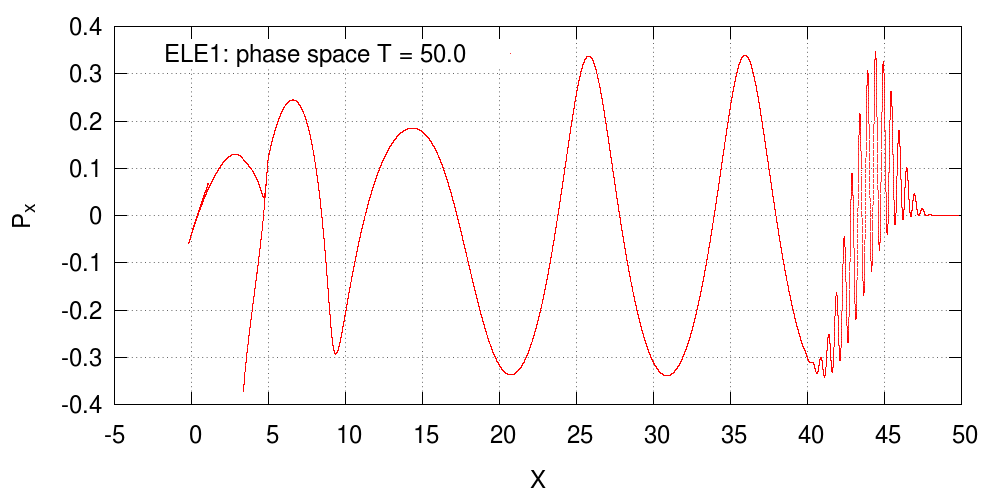
\includegraphics[width=0.80\textwidth]{wake.png}
    \caption{1D wakefield: electrons phase space}
	\label{pic_1dwake}    
    \end{figure}    

\section{1D simple TNSA simulation}
\begin{center}
    \begin{tabular}{ l | l }
    	\textbf{main file name} & \verb+1d_TNSA.cpp+\\
    	\textbf{short description} & simple simulation of TNSA ion acceleration\\
    	\textbf{dimensionality} & 1D  \\
    	\textbf{expected execution time} & around 1 minute on a modern machine (4 MPI processes)
    \end{tabular}
    \end{center}
A P polarized laser pulse with a normalized amplitude of 8.0 interacts with a thin (1.5 $\lambda$) carbon target(``ION1''). There's a very thin layer of hydrogen contaminants on the rear side of the target.\\
Picture \ref{pic_1dTNSA} shows the phase space of carbon ions.
    
    
    \begin{figure}[htbp]
    \centering
    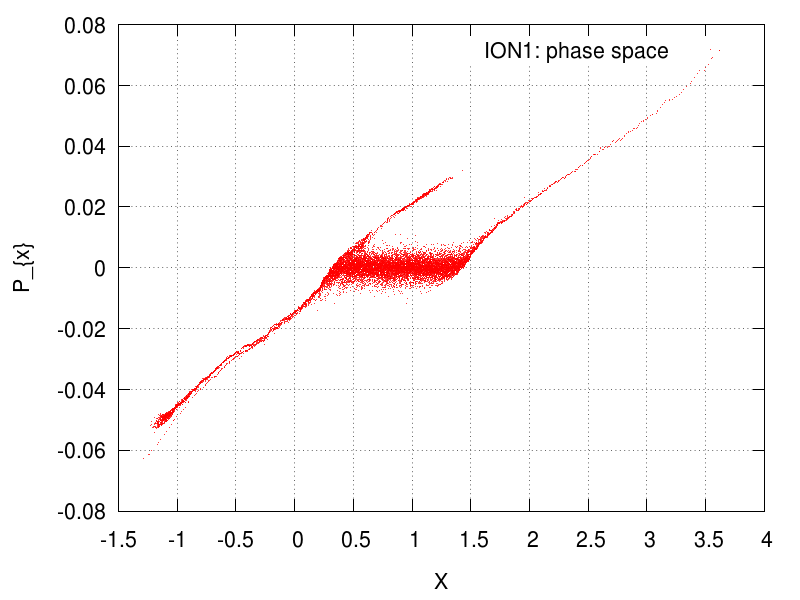
\includegraphics[width=0.80\textwidth]{TNSA1d.png}
    \caption{1D TNSA: ion1 phase space}
	\label{pic_1dTNSA}    
    \end{figure}    

\section{2D grating with stretched grid and 2 laser pulses}
\begin{center}
    \begin{tabular}{ l | l }
    	\textbf{main file name} & \verb+2d_grating.cpp+\\
    	\textbf{short description} & two laser pulses  a grating target \\
    	\textbf{dimensionality} & 2D  \\
    	\textbf{expected execution time} & around 1.5 hours on a supercomputer (1024 MPI processes on a BG/Q)
    \end{tabular}
    \end{center}
In this simulations, two inclined laser pulses interact with an overdense grating target. \\
Several features of emph{piccante} code are used in this simulation, such as the stretched grid, complex target shapes and multiple laser pulses. Figure \ref{pic_2dgrt} shows the initial setup of this simulation.

\begin{figure}[htbp]
        \centering
          \begin{subfigure}[c]{0.3\textwidth}
                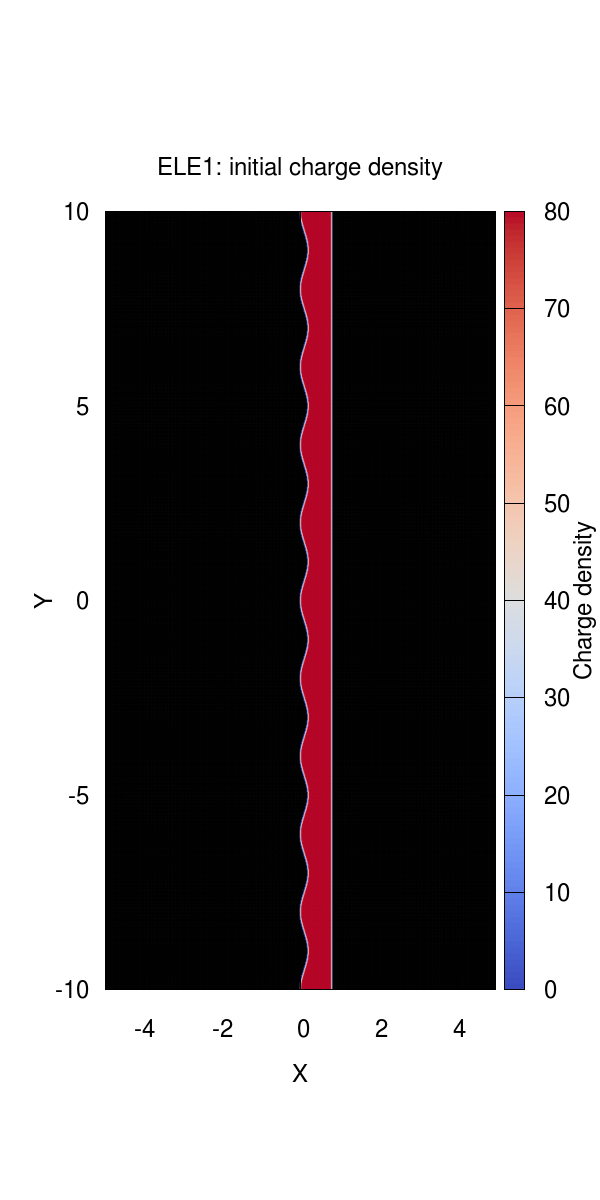
\includegraphics[width=\textwidth]{2d.png}                
                
        \end{subfigure}
                  \begin{subfigure}[c]{0.4\textwidth}
                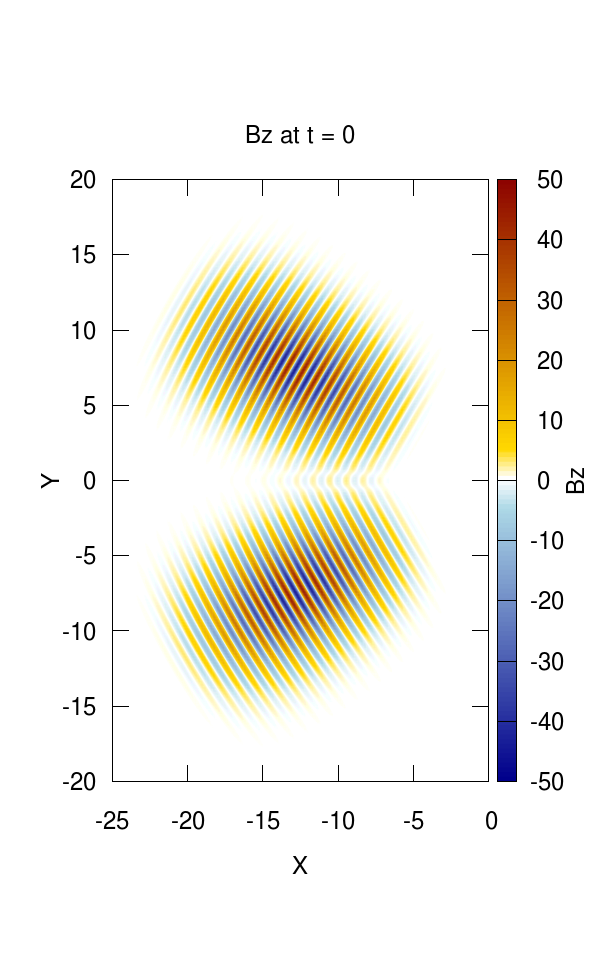
\includegraphics[width=\textwidth]{2d_field.png}                
                
        \end{subfigure}
        \caption{2D grating: The initial setup (target and Bz field component)}
        \label{pic_2dgrt}
\end{figure}

\section{3D two stream instability}
\begin{center}
    \begin{tabular}{ l | l }
    	\textbf{main file name} & \verb+3d_twostream.cpp+\\
    	\textbf{short description} & two counter-streaming electron clouds \\
    	\textbf{dimensionality} & 3D  \\
    	\textbf{expected execution time} & several hours on a supercomputer (1024 MPI processes on a BG/Q)
    \end{tabular}
    \end{center}
In this simulation there are two counter-streaming electron clouds with normalized momentum along z equal to 1. There is a very small initial temperature. \\
An instability develops and a significant fraction of the initial kinetic energy is converted into EM field energy.   \\
Figure \ref{pic_3dtwostream} shows the charge density of one of the electron species after a few plasma periods.
 \begin{figure}[htbp!]
    \centering
    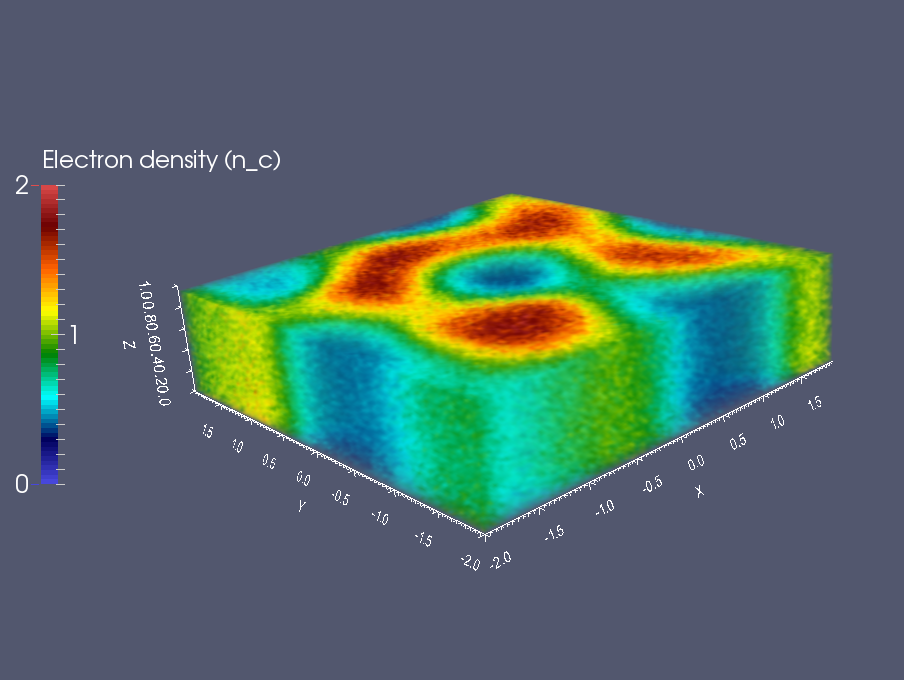
\includegraphics[width=0.70\textwidth]{3d_marta.png}
    \caption{3D twostream: development of the instability(ELE1 charge density)}
	\label{pic_3dtwostream}    
\end{figure}    

 

\chapter*{Appendix A: code normalization}
\tikz[remember picture,overlay] {%
\draw [bordercolor,line width=10mm]
(current page.south west)
rectangle
(current page.north east)
;}Everything in the code scales with $\ell_0$ scale-length.\\
$m_e$ and $q_e$ are, respectively, the mass and the charge of an electron, while $c$ is the speed of light.
\section*{Normalization of code quantities}
\begin{eqnarray*}
q &=& \widetilde{q} \: q_e\\
m &=& \widetilde{m} \: m_e\\
\mathbf{E} &=& \widetilde{\mathbf{E}} \: \dfrac{m_e c^2}{q_e \ell_0} \\
\mathbf{B} &=& \widetilde{\mathbf{B}} \: \dfrac{m_e c^2}{q_e \ell_0} \\
t &=& \widetilde{t} \: \dfrac{\ell_0}{c} \\
l &=& \widetilde{l} \: \ell_0 \\
\mathbf{p} &=& \widetilde{\mathbf{p}} \widetilde{m} \: m_e c \\
\mathbf{v} &=& \widetilde{\mathbf{v}} \: c \\
\mathbf{J} &=& \widetilde{\mathbf{J}} \: \dfrac{m_e c^3 \pi}{q_e \ell_0}
\end{eqnarray*}
\section*{Normalized Particle equations}
$$
\begin{cases}
    \partial_{\widetilde{t}} \widetilde{p} = & \dfrac{\widetilde{q}}{\widetilde{m}} \left({\widetilde{\mathbf{E}} + \widetilde{\mathbf{v}} \times \widetilde{\mathbf{E}}}\right) \\
   \widetilde{\mathbf{J}} = & \widetilde{q} \sum_n{\dfrac{W_n}{\Delta \widetilde{V}} \widetilde{\mathbf{v}}_n} \\
\end{cases}
$$

\section*{Normalized Maxwell equations}
$$
\begin{cases}
    \partial_{\widetilde{t}} \widetilde{\mathbf{B}} = & - \widetilde{\nabla} \times \widetilde{\mathbf{E}} \\
    \partial_{\widetilde{t}} \widetilde{\mathbf{E}} = & \widetilde{\nabla} \times \widetilde{\mathbf{B}} - 4\pi^2 \widetilde{\mathbf{J}}
\end{cases}
$$

\end{document}

